\documentclass{beamer}
\mode<presentation>
{
  \usetheme{ldv}
  \setbeamercovered{transparent}
}

% Uncomment this if you're giving a presentation in german...
\usepackage[ngerman]{babel}

% ...and rename this to "Folie"
\newcommand{\slidenomenclature}{Folie}


\usepackage[utf8]{inputenc}
\usepackage{amsmath,amssymb,amsfonts}
\usepackage{times}
\usepackage{graphicx}
\usepackage{fancyvrb}
\usepackage{array}
\usepackage{colortbl}
\usepackage{tabularx}

% Uncomment me when you need to insert code
\usepackage{color}
\usepackage{listings}
\usepackage{minted}
\usepackage{algpseudocode}
% End Code

\usepackage{datetime}

% Uncomment me when you need video or sound
% \usepackage{multimedia}
% \usepackage{hyperref}
% End video

% Header
\newcommand{\zwischentitel}{Tutorium 1}
\newcommand{\leitthema}{Tobias Eppacher}
\newcommand{\presdatum}{\formatdate{5}{5}{2025}}
% End Header

% Titlepage
\title{Grundlagen: Algorithmen und Datenstrukturen}
\author{Tobias Eppacher}
\date{\presdatum}
\institute{School of Computation, Information and Technology}
\subtitle{Tutorium 1}
% End Titlepage


% Slides
\begin{document}

% 1. Slide: Titlepage
\begin{frame}
	\titlepage
\end{frame}

% 2. Slide: TOC
\begin{frame}
	\frametitle{Table of contents}
	\tableofcontents[subsectionstyle=hide]
\end{frame}

% Further Slides
\section{Organisation}

\begin{frame}
	\frametitle{Organisation}
	\begin{figure}
		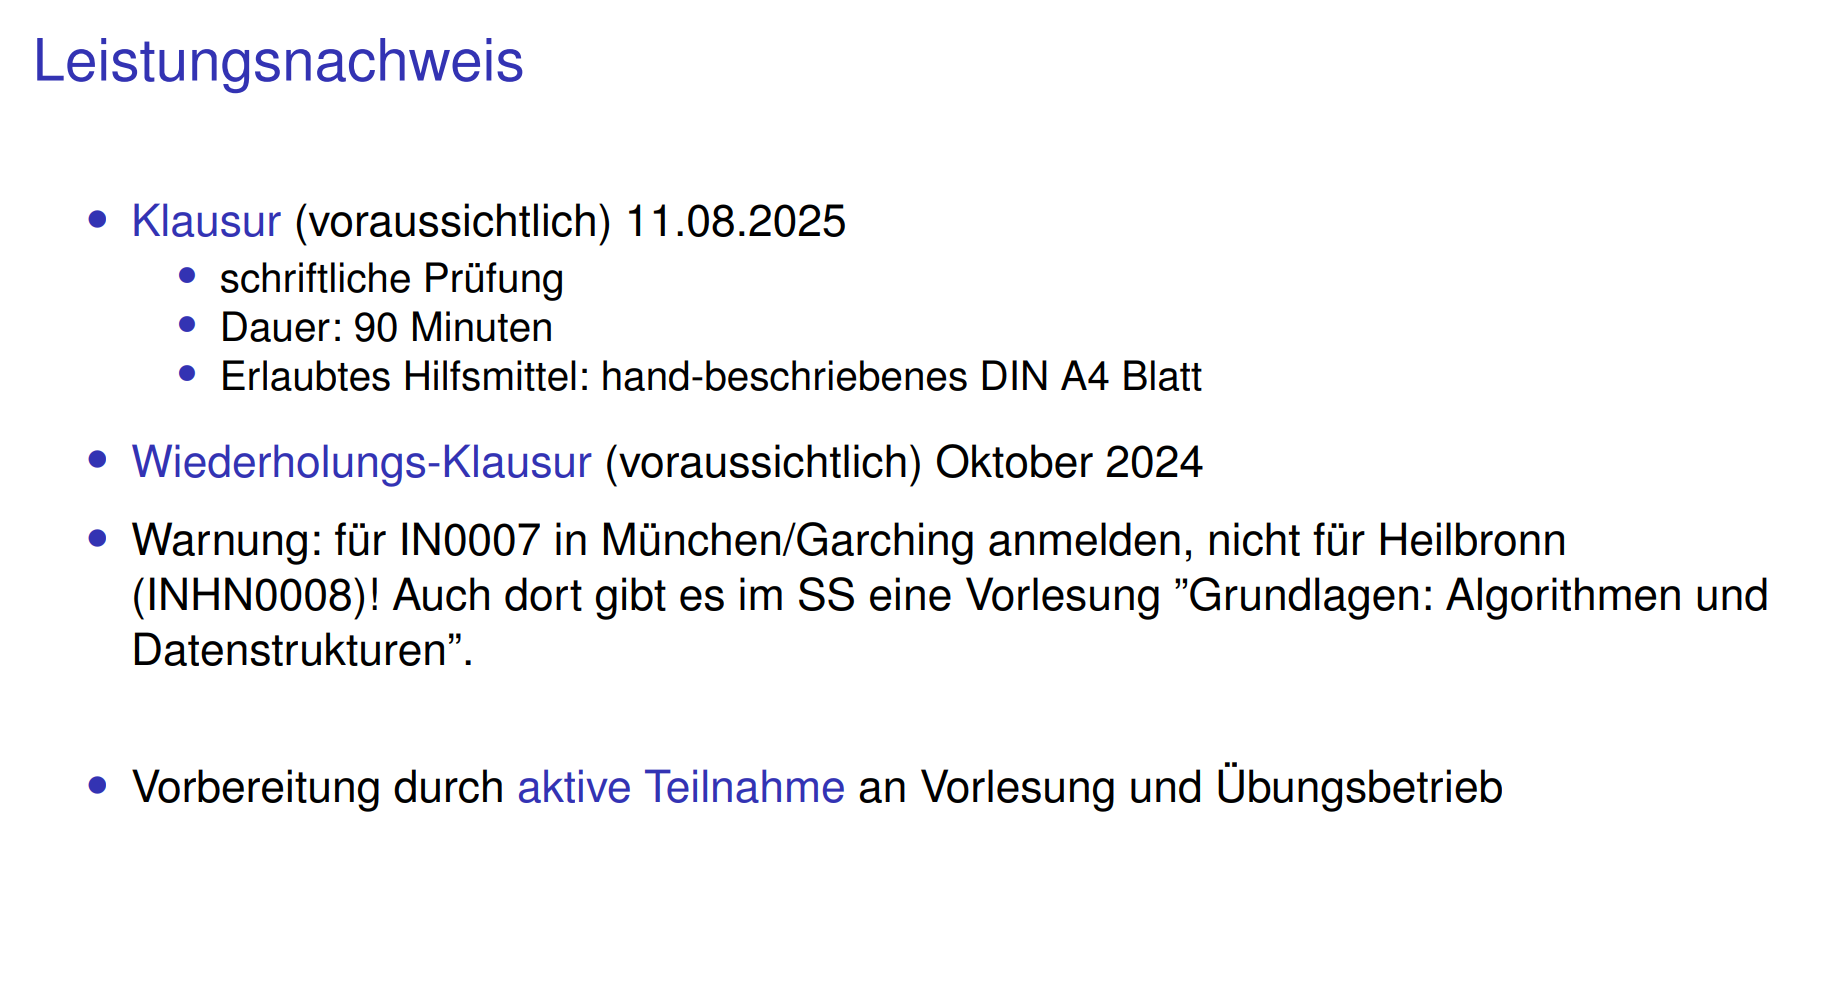
\includegraphics[width=\textwidth]{images/orga.png}
		\caption{Aus den Vorlesungsfolien}
	\end{figure}
\end{frame}

\begin{frame}
	\frametitle{Zulip}
	Kommunikation über Zulip (\url{https://zulip.in.tum.de/})

	\begin{figure}
		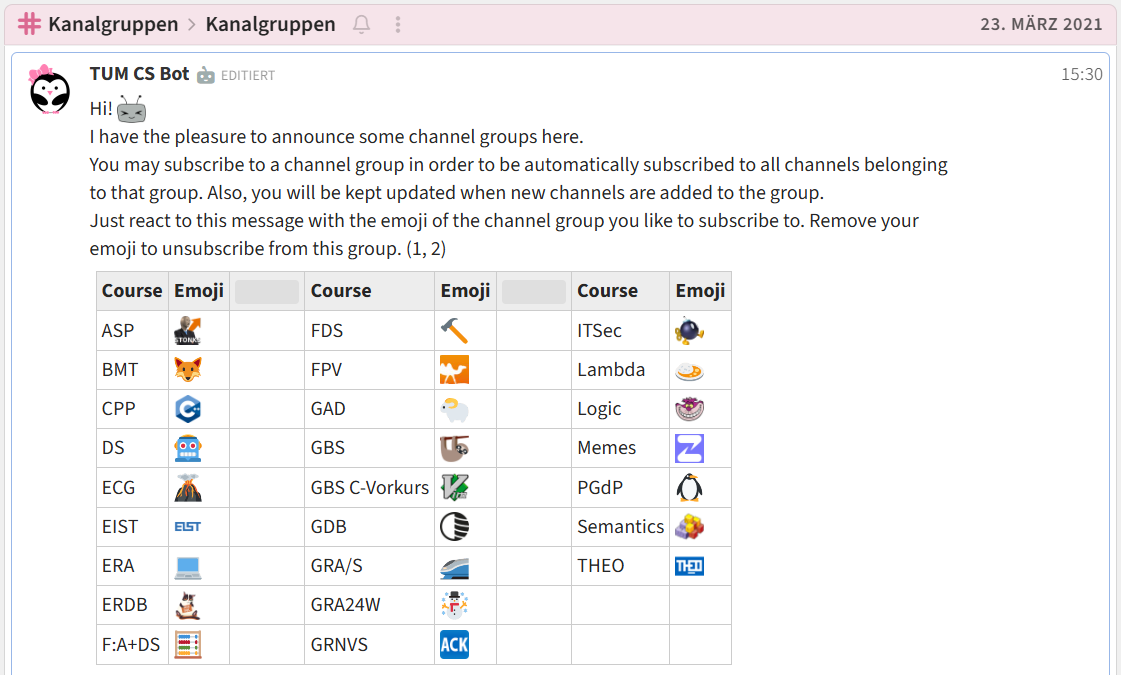
\includegraphics[width=0.9\textwidth]{images/zulip-groups.png}
	\end{figure}
\end{frame}

\begin{frame}
	\frametitle{Zulip}
	Tutoriumschannels:

   \begin{enumerate}
      \item Montag 14:00: GAD Tutorium A-14-4
      \item Montag 16:00: GAD Tutorium A-16-5
   \end{enumerate}

   Zulip DM an mich (Tobias Eppacher) für nicht öffentliche Fragen oder Feedback :)
\end{frame}



\section{Aufgaben}

\subsection{Division}
\begin{frame}
	\frametitle{Aufgabe 1.1 - Division}
	\begin{columns}[T]

		\begin{column}{.57\textwidth}
			\textbf{Input:} Ziffer$[](x_1, x_2, \dots, x_n)$, Ziffer $y$
			\begin{algorithmic}[1]
				\State int $i := 1$
				\State Ziffer $x_0 := 0$
				\While{$i \leq n$}
				\If{$x_{i-1} > 0$}
				\State Ziffer $z_i := g(x_{i-1} \oplus  x_i, y)$
				\State $x_i := r(x_{i_1} \oplus x_i, y)$
				\State $x_{i-1} := 0;$
				\Else
				\State Ziffer $zi := g(xi, y)$
				\State $xi := r(xi, y)$
				\EndIf
				\State $i := i + 1$
				\EndWhile
			\end{algorithmic}
		\end{column}
		\begin{column}{.41\textwidth}

			\textbf{Grundoperationen:}
			\begin{itemize}
				\item $g(x, y)$ Ganzzahldivision
				\item $r(x, y)$ Rest
				\item $+$ Addition
				\item $:=$ Zuweisung
				\item $>, <, \dots$ Vergleich
			\end{itemize}
			\textit{Indexberechnung keine Grundoperation}
		\end{column}
	\end{columns}
\end{frame}

\begin{frame}
	\frametitle{Aufgabe 1.1 - Division}
	Wie viele Grundoperationen hat die Schulmethode in unserem Rechenmodell im schlimmsten
	Fall, wenn man eine Zahl mit $n$ Ziffern ganzzahlig durch eine Ziffer teilt? Betrachten Sie bei
	Ihrer Lösung jeweils jede Zeile im Pseudocode.
\end{frame}

\begin{frame}
	\frametitle{Aufgabe 1.1 - Division}
	\begin{algorithmic}[1]
		\State int $i := 1$
		\State Ziffer $x_0 := 0$
		\While{$i \leq n$}
		\If{$x_{i-1} > 0$}
		\State Ziffer $z_i := g(x_{i-1} \oplus  x_i, y)$
		\State $x_i := r(x_{i_1} \oplus x_i, y)$
		\State $x_{i-1} := 0;$
		\Else
		\State Ziffer $zi := g(xi, y)$
		\State $xi := r(xi, y)$
		\EndIf
		\State $i := i + 1$
		\EndWhile
	\end{algorithmic}
\end{frame}


\subsection{Induktion}
\begin{frame}
	\frametitle{Aufgabe 1.2 - Induktion}
	\textbf{Induktionsbeweis} \\
	Zu beweisende Aussage, z.B. $\forall n \in \mathbb{N}: P(n)$
	\begin{enumerate}
		\item Induktionsanfang  \\ zeige Aussage für Basisfall, z.B. $n=1$ für $\mathbb{N}$
		\item Induktionsannahme \\ z.B. $P(n)$ gilt für ein beliebiges, frei gewähltes $n \in \mathbb{N}$
		\item Induktionsschritt  \\ zeige $P(n+1)$ mithilfe der Annahme $P(n)$
	\end{enumerate}
\end{frame}

\begin{frame}
	\frametitle{Aufgabe 1.2 (a)}
	Zeigen Sie für alle natürlichen Zahlen $n \geq 1$ mittels Induktion die folgende Behauptung: \\
	\medskip
	Die Summe der ersten $n$ ungeraden Zahlen ist $n^2$ \\
	(als Formel: $\sum_{i=1}^{n}(2i-1) = n^2$) \\
	\medskip
	Kennzeichnen bzw. benennen Sie in Ihrem Beweis den Induktionsanfang, die Induktionsvoraussetzung und den Induktionsschritt.
\end{frame}

\begin{frame}
	\frametitle{Aufgabe 1.2 (a)}
\end{frame}

\begin{frame}
	\frametitle{Aufgabe 1.2 (b)}
	Zeigen Sie \\
	\smallskip
	$F_{n+1}F_{n-1} - F_n^2 = (-1)^n$, \\
	\smallskip
	wobei $F_n$ die $n$-te Fibonaccizahl nach der rekursiven Definition $F_n = F_{n-1} + F_{n-2}$
	mit den Anfangswerten $F_0 = 0$ und $F_1 = 1$ ist.
\end{frame}

\begin{frame}
	\frametitle{Aufgabe 1.2 (b)}
\end{frame}

\subsection{Bubblesort mit Listen}
\begin{frame}[fragile]
	\frametitle{Aufgabe 1.3 - Bubblesort mit Listen}
	\begin{columns}
		\begin{column}[t]{0.48\textwidth}
			\begin{minted}[fontsize=\tiny]{java}
public class List {

   private static class Node {
      private int data;

      public int getData() {
         return data;
      }

      public void setData(int data) {
         this.data = data;
      }

      private Node next;

      public Node getNext() {
         return next;
      }

      public Node(int data, Node next) {
         this.data = data;
         this.next = next;
      }
   }
        \end{minted}
		\end{column}

		\begin{column}[t]{0.48\textwidth}
			\begin{minted}[fontsize=\tiny]{java}
   private Node head;
   private int size;

   public int getSize() {
      return size;
   }

   public List() {}

   public void prepend(int data) {
      head = new Node ( data , head );
      size ++;
   }

   public int get(int index) {
      Node it = head;
      while(index != 0) {
         index--;
         it = it.getNext ();
         if(it == null) 
            throw new RuntimeException("Out of bounds");
      }
      return it.getData();
   }
        \end{minted}
		\end{column}
	\end{columns}
\end{frame}

\begin{frame}[fragile]
	\frametitle{Aufgabe 1.3 - Bubblesort mit Listen}
	\begin{minted}[fontsize=\tiny]{java}
   public void swap(int indexFirst, int indexSecond) {
      if(head == null) {
         throw new RuntimeException("Out of bounds");
      }

      if(indexFirst > indexSecond) {
         swap(indexSecond, indexFirst);
         return;
      }

      int distance = indexSecond - indexFirst;
      Node it_first = head;

      while(indexFirst != 0) {
         indexFirst--;
         it_first = it_first.getNext();
         if(it_first == null) throw new RuntimeException("Out of bounds");
      }

      Node it_second = it_first;
      while(distance != 0) {
         distance--;
         it_second = it_second.getNext();
         if(it_second == null) throw new RuntimeException("Out of bounds");
      }

      int temp = it_second.getData();
      it_second.setData(it_first.getData());
      it_first.setData(temp);
   }
}
   \end{minted}
\end{frame}


\begin{frame}
	\frametitle{Aufgabe 1.3 - Bubblesort mit Listen}
	\textbf{Implementierung}
	\begin{enumerate}
		\item Welche der Methoden sind langsam, welche schnell? Wieso?
		\item Die \textit{swap}-Methode ruft sich selbst auf. Wie nennt man Methoden, die sich so verhalten?
		      Welche Motivationen gibt es, derart zu programmieren? Welche Nachteile hat so ein Ansatz?
	\end{enumerate}
\end{frame}

\begin{frame}[fragile]
	\frametitle{Aufgabe 1.3 - Bubblesort mit Listen}
	\begin{minted}[fontsize=\tiny]{java}
void bubblesort ( List l) {
   for(int i = 0; i < l.getSize(); i++)
      for(int j = 1; j < l.getSize() - i; j++)
         if(l.get(j - 1) > l.get(j))
            l.swap(j - 1, j);
}
         \end{minted}
	\begin{enumerate}
		\item Die Methode hat keinen Rückgabewert; funktioniert sie dennoch? Wenn ja, wieso?
		\item Wie funktioniert der Algorithmus, warum liefert er stets ein sortiertes Ergebnis?
	\end{enumerate}
\end{frame}

\begin{frame}[fragile]
	\frametitle{Aufgabe 1.3 - Bubblesort mit Listen}
	\begin{minted}[fontsize=\tiny]{java}
void bubblesort (List l) {
   for(int i = 0; i < l.getSize(); i++)
      for(int j = 1; j < l.getSize() - i; j++)
         if(l.get(j - 1) > l.get(j))
            l.swap(j - 1, j);
}
         \end{minted}
	\begin{enumerate}
		\setcounter{enumi}{2}
		\item Wie oft ungefähr wird eine Liste der Größe $n$ durchlaufen? \\
		      \textit{Berücksichtigen Sie bei Ihrer Antwort nur die Implementierung des Bubblesort-Algorithmus}.
		\item Eignet sich unsere Implementierung einer Liste hier besonders gut oder besonders schlecht? \\
		      \textit{Ziehen Sie nun die Implementierung der Listenmethoden in Ihre Laufzeitüberlegung mit ein.}
	\end{enumerate}
\end{frame}

\begin{frame}
	\frametitle{Aufgabe 1.3 - Bubblesort mit Listen}
   Ein bisschen PGdP :) \\

	\begin{enumerate}
		\item Was hat es mit der Schachtelung der Klassen auf sich?
		\item Wozu wurde der Wrapper \mintinline{java}{List} implementiert, statt den Benutzer direkt auf Knoten
		      arbeiten zu lassen? Was hat dies mit \textit{abstrakten Datentypen} zu tun?
		\item Welchen Zweck erfüllt \mintinline{java}{throw}? Wieso ist dies besser, als vordefinierte Fehlerwerte
		      zurückzugeben?
		\item Vergleichen Sie die Implementierung der Funktionen \mintinline{java}{get} und \mintinline{java}{swap}.
		      Was fällt Ihnen dabei auf? Wann kann das ein Problem sein, und wie lässt sich dieses vermeiden?
	\end{enumerate}
\end{frame}

\section{E-Aufgaben}
\begin{frame}
	\frametitle{E-Aufgaben}
	\begin{itemize}
		\item Aufgabe 1.4 - Tiefe Bäume \\
		      \begin{itemize}
			      \item Definitionen zum Thema Bäume
			      \item Übung zu Induktion
		      \end{itemize}
		\item Aufgabe 1.5 - Schwere Induktion
		      \begin{itemize}
			      \item Schwerer Induktionsbeweis
			      \item Ebenfalls gute Übung
		      \end{itemize}
	\end{itemize}
\end{frame}

\section{Hausaufgaben}
\begin{frame}
	\frametitle{Hausaufgaben}
	\begin{itemize}
		\item Hausaufgaben auf Artemis (\url{https://artemis.tum.de/})
	\end{itemize}
	\begin{enumerate}
		\item Hausaufgabe 1: Labyrinth (Deadline - 07.05.2025)
		\item Hausaufgabe 2: Binäre Suche (Deadline - 14.05.2025)
	\end{enumerate}
\end{frame}

\begin{frame}
	\textbf{Fragen?}
	\begin{itemize}
		\item Nach Übung gerne bei mir melden
		\item Tutoriumschannel oder DM an mich auf Zulip
		\item Vorlesungschannels von GAD auf Zulip (insbesondere bei Hausaufgaben)
	\end{itemize}

	\medskip
	\textbf{Feedback oder Verbesserungsvorschläge?} \\
	Gerne nach dem Tutorium mit mir quatschen oder DM auf Zulip

	\medskip
	\textbf{Bis nächste Woche!}
\end{frame}

% End Slides

\end{document}
